% Created 2011-08-25 Thu 13:04
\documentclass[11pt,english]{article}
\usepackage[utf8]{inputenc}
\usepackage[T1]{fontenc}
\usepackage{fixltx2e}
\usepackage{graphicx}
\usepackage{longtable}
\usepackage{float}
\usepackage{wrapfig}
\usepackage{soul}
\usepackage{textcomp}
\usepackage{marvosym}
\usepackage{wasysym}
\usepackage{latexsym}
\usepackage{amssymb}
\usepackage{hyperref}
\tolerance=1000
\usepackage{color}
\usepackage{listings}

\usepackage{lmodern}
\renewcommand{\sfdefault}{lmss}
\renewcommand{\ttdefault}{lmtt}

% needed packages
\usepackage{amsmath}
\usepackage{amssymb}
\usepackage{amsthm}
\usepackage{babel}
\usepackage{epsfig}
\usepackage[T1]{fontenc}
\usepackage{fixltx2e}
\usepackage{float}
%\usepackage{floatflt}
\usepackage{graphics}
\usepackage{graphicx}
\usepackage[utf8]{inputenc}
\usepackage{latexsym}
\usepackage{longtable}
\usepackage{makeidx}
\usepackage{marvosym}
\usepackage{multicol}
%\usepackage{pslatex}
\usepackage{rotating}
%\usepackage{showidx}
\usepackage{soul}
\usepackage{srcltx}
\usepackage{stmaryrd}
\usepackage{subfig}
\usepackage{textcomp}
%\usepackage{theorem}
%\usepackage[subfigure]{tocloft}
\usepackage{txfonts}
\usepackage{upgreek}
\usepackage{url}
\usepackage{varioref}
%\usepackage{wasysym}
\usepackage{wrapfig}


% Page setup
\usepackage[paperwidth=8.5in,paperheight=11in]{geometry}
\geometry{verbose,tmargin=0.5in,bmargin=0.5in,lmargin=1in,rmargin=1in}




% PDF settings
%\usepackage[hyperref,x11names]{xcolor}
\usepackage{hyperref}
\hypersetup{pdftitle={STAT 5840: Statistical Computing},
 		pdfauthor={G. Jay Kerns}, 
		linkcolor=Firebrick4, 
		citecolor=black, 
		urlcolor=SteelBlue4}

% Listings setup
%\usepackage{color}
%\usepackage{listings}
%\lstset{basicstyle={\ttfamily},
%	language=R,
%	breaklines=true,
%	breakatwhitespace=true,
%	keywordstyle={\ttfamily},
%	numberstyle = {\ttfamily},
%	morestring=[b]"
%}



%  user defined commands
% special operators
\renewcommand{\P}{\mathrm{I\hspace{-1.5pt}P}}
\newcommand{\E}{\mathrm{I\hspace{-1.5pt}E}}
\renewcommand{\vec}[1]{\mbox{\boldmath$#1$}}

% special symbols
\newcommand{\me}{\mathrm{e}}
\newcommand{\R}{\mathbb{R}}
\newcommand{\diff}{\mathrm{d}}
\newcommand{\ybar}{\overline{y}}
\newcommand{\xbar}{\overline{x}}
\newcommand{\Xbar}{\overline{X}}
\newcommand{\Ybar}{\overline{Y}}





\providecommand{\alert}[1]{\textbf{#1}}

\title{Bayesian Monte Carlo Computations}
%\author{G. Jay Kerns}
\date{STAT 5840: Summer 2011}

\begin{document}

\maketitle

\thispagestyle{empty}

\section*{Estimating a Normal mean with a Cauchy Prior}
\label{sec-1}

We would like to illustrate using the Monte Carlo method to estimate complicated integrals in Bayesian applications.  The following is a script which estimates the mean of a Normal distribution when our prior distribution is Cauchy.


\begin{verbatim}
# cauchyprior.R
set.seed(1) # make the experiment reproducible
m <- 2000   # number of simulated values
x <- 3      # observed data

# Now simulate some random variables
theta <- rcauchy(m) # simulate m standard Cauchys
h <- pi*exp(-0.5*(x-theta)^2)  # compute h(theta)

C <- mean(h)  # estimate the normalizing constant
post.mean <- mean(theta*h)/mean(h) # estimate the posterior mean

# We'd like to see a running average plot to assess convergence

num <- theta*h   # vector in the numerator
rc <- rep(0, times = m)
rpm <- rep(0, times = m)

for (i in seq.int(m)){         # seq.int(m) will be 1:m
  rc[i] <- mean(h[1:i])
  rpm[i] <- mean(num[1:i])/mean(h[1:i])
}
\end{verbatim}
\section*{At the command prompt}
\label{sec-2}



\begin{verbatim}
C
post.mean
\end{verbatim}




\begin{verbatim}
 [1] 0.3724711
 [1] 2.334232
\end{verbatim}


The true values are \(C \approx 0.34168057 \) and \(\mbox{Posterior Mean} = 2.284967653\).


\begin{verbatim}
# now plot the results
par(mfrow = c(1,2))
plot(3:200, rpm[3:200], type = "l", ylim = c(0, 2.7))
lines(3:200, rc[3:200], type = "l")
plot(1:m, rpm, type = "l", ylim = c(0, 2.7))
lines(1:m, rc, type = "l")
par(mfrow = c(1,1))
\end{verbatim}




\begin{figure}[h!]
\centering
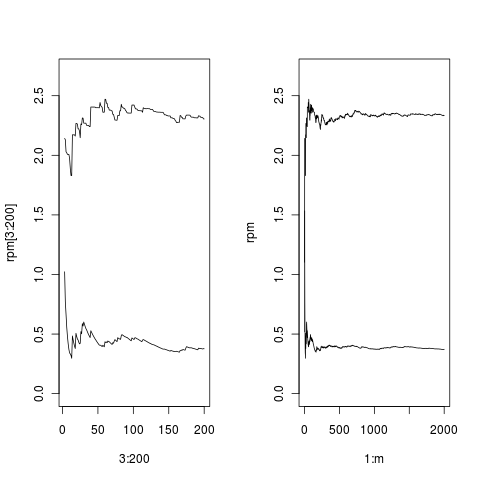
\includegraphics[width=6in, height=6in,]{img/CauchyPrior.pdf}
\caption{\label{fig:yplot}Running averages for assessing convergence of the estimators}
\end{figure}

\end{document}